\documentclass{beamer}
\usetheme{Madrid}
\usecolortheme{default}

\usepackage{caption}
\captionsetup[algorithm]{font=tiny}
\usepackage{algorithm}
% \SetAlFnt{\small}
% \SetAlCapFnt{\tiny}
% \SetAlCapNameFnt{\tiny}
\usepackage{algorithmic}
\algsetup{linenosize=\tiny}
\usepackage{float}

\def\R{\mathrm{R}}
\def\Z{\mathbb{Z}}
\def\N{\mathbb{N}}
\def\S{\mathbb{S}}
\def\I{\mathbb{I}}
\def\P{\mathbb{P}}
\def\s{\mathbf{s}}
\def\a{\mathbf{a}}
\def\r{\mathbf{r}}

\newtheorem{thm}{Theorem}[]
%\numberwithin{thm}{section} 
\newtheorem{assm}[]{Assumption}
\newtheorem{lem}[]{Lemma}
\newtheorem{prop}[]{Proposition}
\def\half{\frac{1}{2}}
\def\onethird{\frac{1}{3}}

\def\tends{\rightarrow}
\def\into{\rightarrow}
\def\implies{\Rightarrow}
\def\is{\leftarrow}
\def\-{\mbox{--}}
\def\e{\epsilon}

\DeclareMathOperator*{\argmin}{arg\,min}
\DeclareMathOperator*{\argmax}{arg\,max}
\usepackage[numbers]{natbib}
% \usepackage[sortcites,style=numeric,sorting=none,backend=biber]{biblatex}
\usepackage{ragged2e}
\usepackage{etoolbox}

\newcommand{\centered}[1]{\begin{tabular}{l} #1 \end{tabular}}
\apptocmd{\frame}{}{\justifying}{}
\usepackage{amsmath}


\title[Mid Prep : Adobe]
{Mid Prep : Adobe}

% \subtitle{Algorithm and Applications}


\author[Team 99] % (optional, for multiple authors)
{Team 99}

\institute[] % (optional)
{
  
  Inter IIT TechMeet 12.0 \\
  % under guidance of \textbf{Dr. Ajin George Joseph}
  
}

\date[Inter IIT Tech Meet] % (optional)
{December, 2023}

% \logo{
\includegraphics[height=0.8cm]{IITTP_LOGO.jpeg}}


\definecolor{uoftblue}{RGB}{6,41,88}
\setbeamercolor{titlelike}{bg=uoftblue}
\setbeamerfont{title}{series=\bfseries}


\begin{document}

\frame{\titlepage}

\begin{frame}
\frametitle{Table of Contents}

\tableofcontents
\end{frame}

\section{Introduction}

\begin{frame}{Introduction to Problem Statement}
\begin{itemize}
    \item The issue statement presented by Adobe comprises two components: behavioral simulation and content simulation.
    \item Firstly, based on the metadata of a given tweet, our task is to forecast the number of likes that particular tweet has received. The evaluation metric used will be the root mean squared error.
    \item To generate the tweet text, utilize the provided tweet metadata including the company, username, media URL, and timestamp. The evaluation of this will be conducted using three metrics: BLEU 1-4, ROUGE, and CIDER.
    \item The test dataset would comprise of two components: an unseen time period and unseen companies.
    
\end{itemize}
% \begin{alertblock}{}
% \begin{itemize}
%     \item The function $f(x)$ might not be fully known i.e. $f(x)$ is not available $\forall x$. 
%     \item The function may not be continuous and differentiable.
% \end{itemize}
% \end{alertblock}

\end{frame}
% \begin{frame}{The Robbins–Monro Algorithm}
%     Suppose for a function, $g(\theta)$, only noise-corrupted observations are available at selected values of $\theta.$ In the above equation (\ref{eq:newton}), $g(\theta_n)$ can be replaced by a good estimate of it by taking many observations.
%     Robbins and Monro\cite{robbins1951stochastic} proposed in 1951 the following update rule:
%     \begin{equation}
%         \label{eq:robinmonro}
%         \theta_{n+1} = \theta_n + \epsilon_n Y_n
%     \end{equation}
%     where, $Y_n$ is a noisy estimate of $g(\theta_n)$ and $\epsilon_n$ is subject to the conditions:
%     \begin{itemize}
%         \item $\epsilon_n>0$, 
%         \item $\epsilon_n \rightarrow 0$,
%         \item $\sum_n \epsilon_n = \infty$,
%         \item $\sum_n \epsilon^2_n < \infty$
%     \end{itemize}
%     e.g. $\epsilon_n = 1/n$, then $\sum_n \frac{1}{n} = \infty$ and $\sum_n \frac{1}{n^2} = \pi^2/6 < \infty$.
%     \end{frame}

    

%     \begin{frame}{Martingale Difference Noise}
%         \begin{block}{Martingale}
%         \scriptsize
%             A sequence of random variables $Y_1,Y_2,\dots,Y_n$ that satisfies for any time $n$ the following:
%             \begin{itemize}
%                 \item $\mathbb{E}(|Y_n|) < \infty $
%                 \item $\mathbb{E}(Y_{n+1}|Y_1,Y_2,\dots,Y_n) = Y_n$
%             \end{itemize}
%             which is the conditional expected value of the next observation, given all the past observations, is equal to the most recent observation.
%         \end{block}
%         \begin{block}{Martingale Difference Series (MDS)}
%         \scriptsize
%             A stochastic series $Y$ is said to be MDS if it's expectation w.r.t it's past is $0$.
%             \begin{itemize}
%                 \item $\mathbb{E}(|Y_t|) < \infty $
%                 \item $\mathbb{E}(Y_{t+1}|Y_1,Y_2,\dots,Y_t) = 0, \forall t$ 
%             \end{itemize}
%             for a sequence $\{Y_t,\mathcal{F}_t\}^\infty_{-\infty}$ on probability space $(\Omega,\mathcal{F},\mathbb{P})$.
%         \end{block}
%     \end{frame}

\section{Solution Pipeline}

\begin{frame}{Solution Pipeline}
% \begin{block}{Theorem}
%     For the given stochastic recursion
% \begin{equation}
% \label{eq:saborkar}
%     Y_{n+1} = Y_n + \alpha_n (h(Y_n) + \mathbb{M}_{n+1})
% \end{equation}
% we have $ \lim_{n\to\infty} Y_n  \in \{y | h(y) = 0\}$ under the following conditions\cite{kushner1997applications}:
% \scriptsize
% \begin{itemize}
%     \item $h$ is linear, $h(x) = Ax + b$ and $A$ is invertible or $h$ is a contraction mapping i.e. $|| h(x) - h(y) ||_{D} < \gamma || x - y ||_{D}$ where $\gamma \in (0,1]$.
%     \item $\{\mathbb{M}_{n+1}\}$ should be martingale difference noise i.e. having zero mean and uncorrelated with any random variable realised up to time $n$.
%     \item $\alpha_{n} \in (0,1) ; \alpha_n \rightarrow 0$ and  $\sum_n \alpha_n = \infty, \sum_n \alpha^2_n < \infty$.
% \end{itemize}
% \end{block}
% where, $Y_n \in \mathbb{R}^k, h:\mathbb{R}^k \rightarrow \mathbb{R}^k $ and $  \mathbb{M}_n \in \mathbb{R}^k$.
\end{frame}

% \begin{frame}{}
%     \scriptsize
%     Say for a r.v. X, whose $p_X$ is unknown to estimate $\mathbb{E}(X)$ we can take $n$ i.i.d samples to get $\mathbb{E}(X) \approx \sum^n_{i=1} \frac{X_i}{n}$.\\
%     Now, let $$S_N = \frac{X_1 + X_2 + \dots + X_n}{n}$$ so $S_N \rightarrow \mathbb{E}(X) \,\,as\,\, n \rightarrow \infty$.
%     Then, $$S_{N+1} = \frac{X_1 + X_2 + \dots + X_n + X_{n+1}}{n+1} \implies S_{N+1} = \frac{n S_N + X_{N+1}}{n+1}$$
%     $$S_{N+1} = (1 - \frac{1}{n+1})S_N + (\frac{1}{n+1})X_{n+1} \implies S_{N+1} = S_N + \frac{1}{n+1}(X_{n+1} - S_N)$$
%     $$S_{N+1} = S_N + \frac{1}{n+1}({\color{red}\mathbb{E}(X) - S_N} + {\color{blue}X_{n+1} - \mathbb{E}(X)})$$
%     which is analogous to the SA form where ${\color{red}h(S_N) = \mathbb{E}(X) - S_N}$ and ${\color{blue}\mathbb{M}_{n+1}=X_{n+1} - \mathbb{E}(X)}$ is a martingale difference noise as $\mathbb{E}(X_{n+1} - \mathbb{E}(X)) = \mathbb{E}(X_{n+1}) - \mathbb{E}(X) = 0.$ (As $X_i$ are i.i.d samples)
%     Also $\sum_n \frac{1}{n+1} = \infty$ and $\sum_n \frac{1}{(n+1)^2} = \frac{\pi^2}{6} < \infty$.
% \end{frame}

% \begin{frame}{}
%         \begin{figure}
%             \centering
%             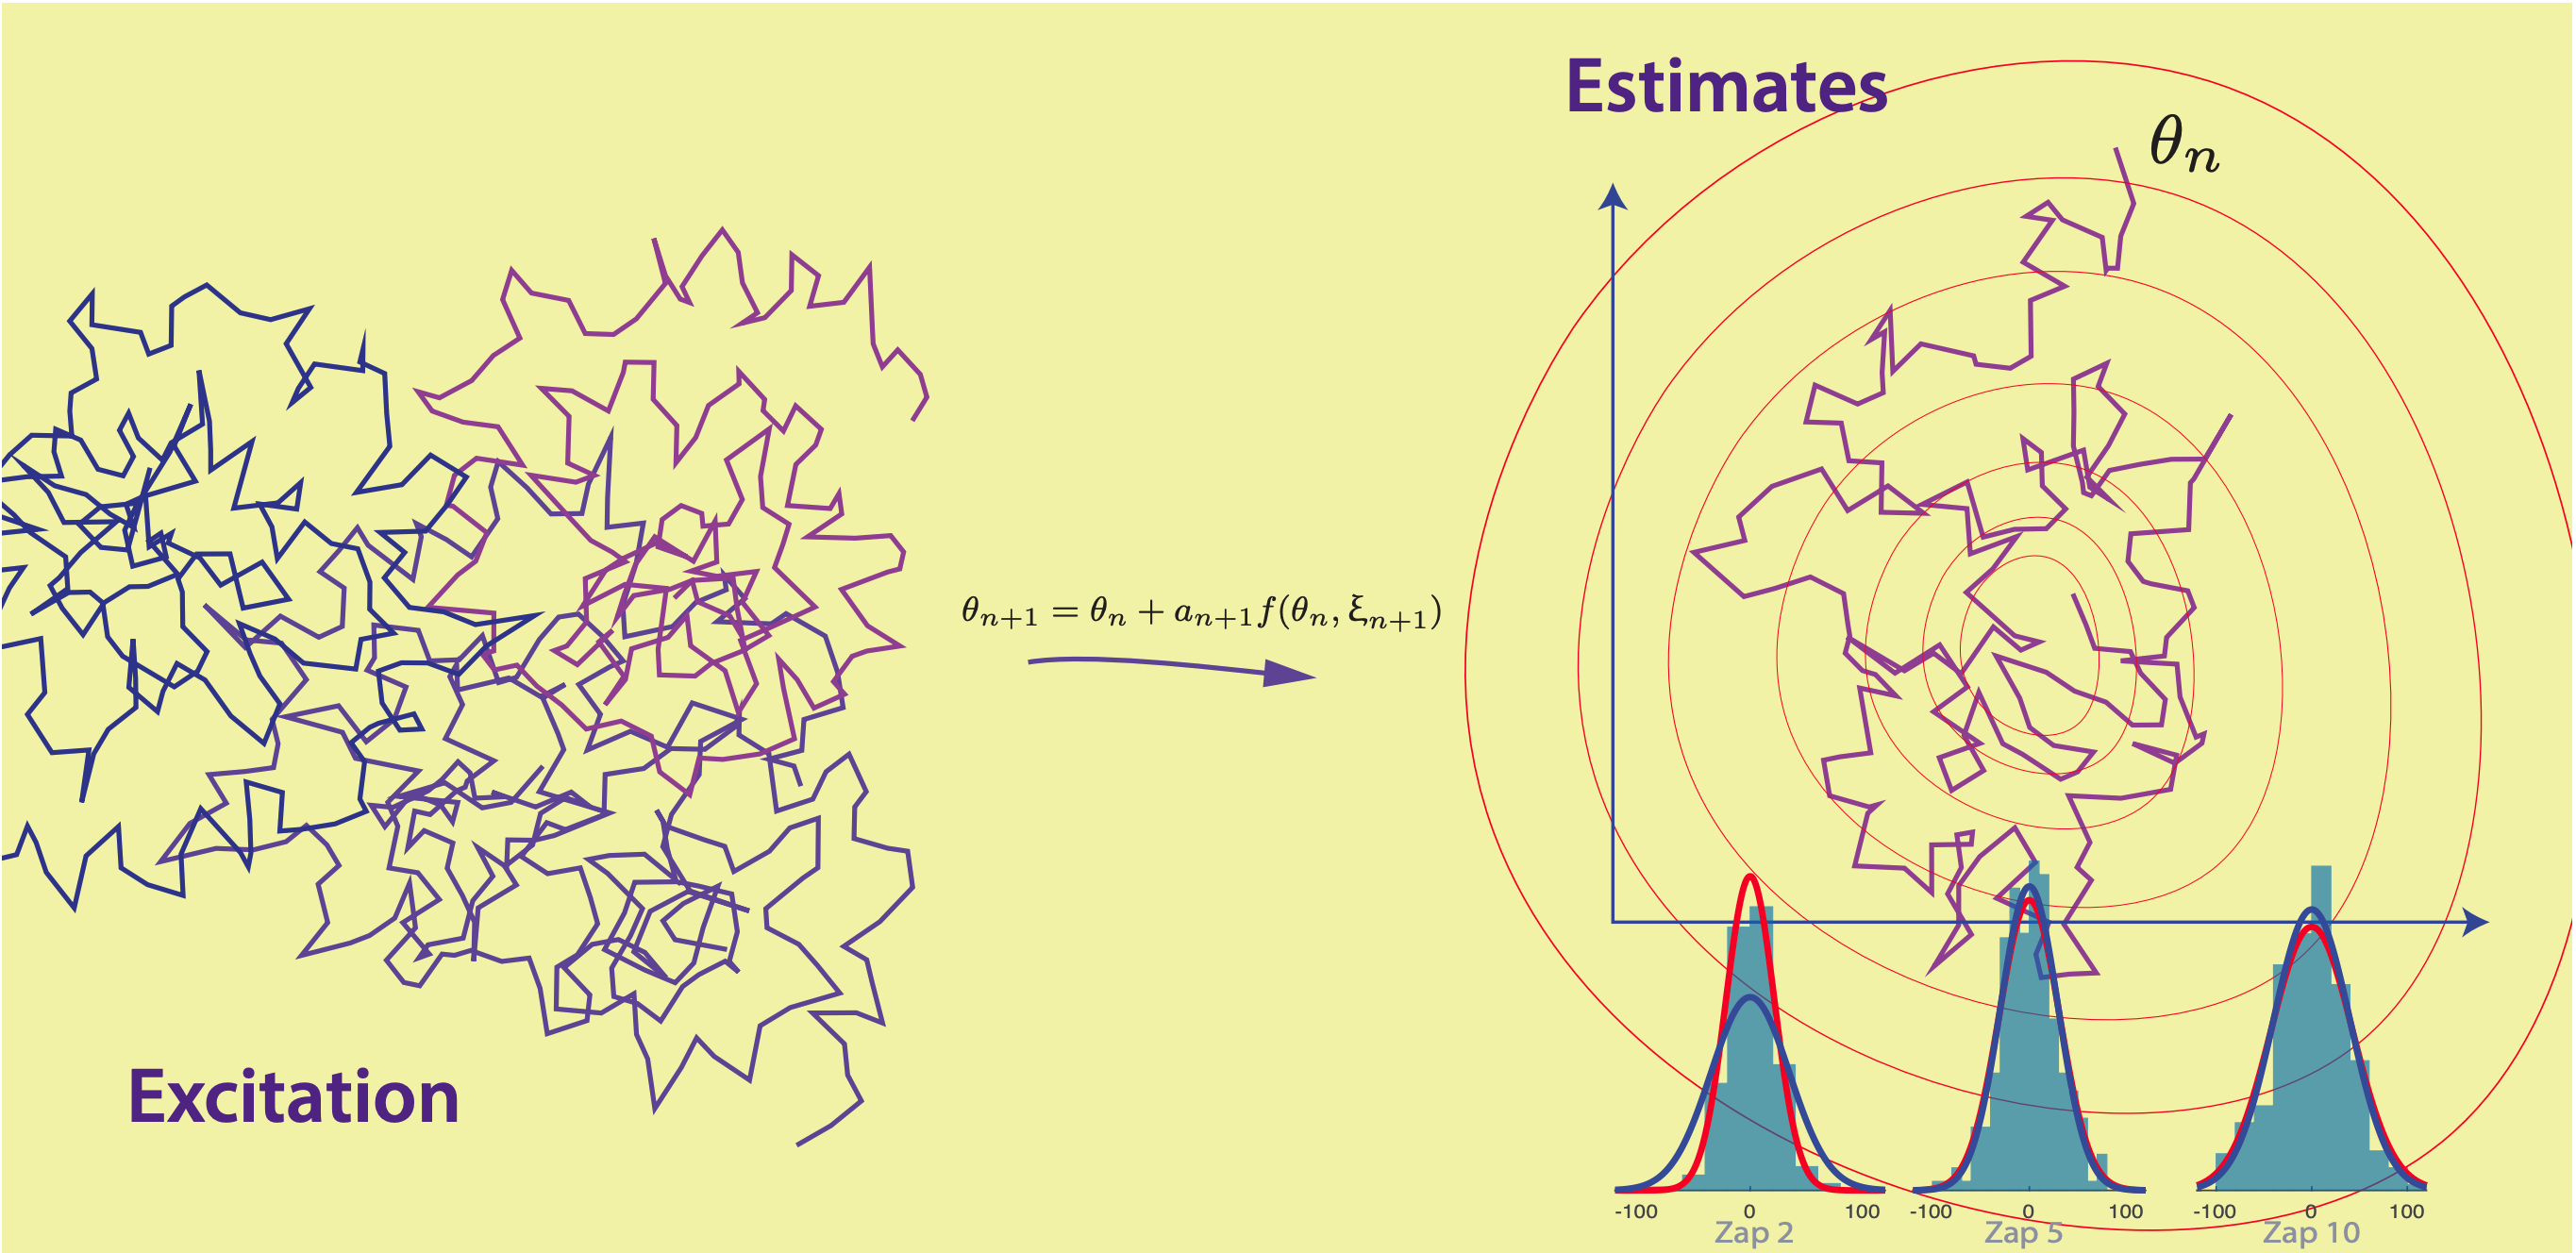
\includegraphics[scale = 0.24]{sa.png}
%             \caption{The generalised idea of stochastic approximation \cite{durand2020zap}}
%             \label{fig:enter-label}
%         \end{figure}
%     \end{frame}

\section{Task 01: Likes Prediction}
\begin{frame}{Task 01: Likes Prediction}
%     \begin{block}{Basic Convergence Analysis}
%         The stochastic recurrence given as $x_{n+1} = x_n + \epsilon_n (h(x_n) + \mathbb{M}_{n+1}); n\geq0 \,\, and \,\, x_0$ can be random and with above assumptions being true and $h(x)$ is Lipschitz continuous then the iterates ${x_n}$ track a.s. asymptotically the ODE \cite{borkar1998stability} $$\dot{x}(t)=h(x(t)), t \geq 0$$
%     \end{block}
% \end{frame}
% \begin{frame}{}
% \begin{figure}
%     \centering
%     \scriptsize
%     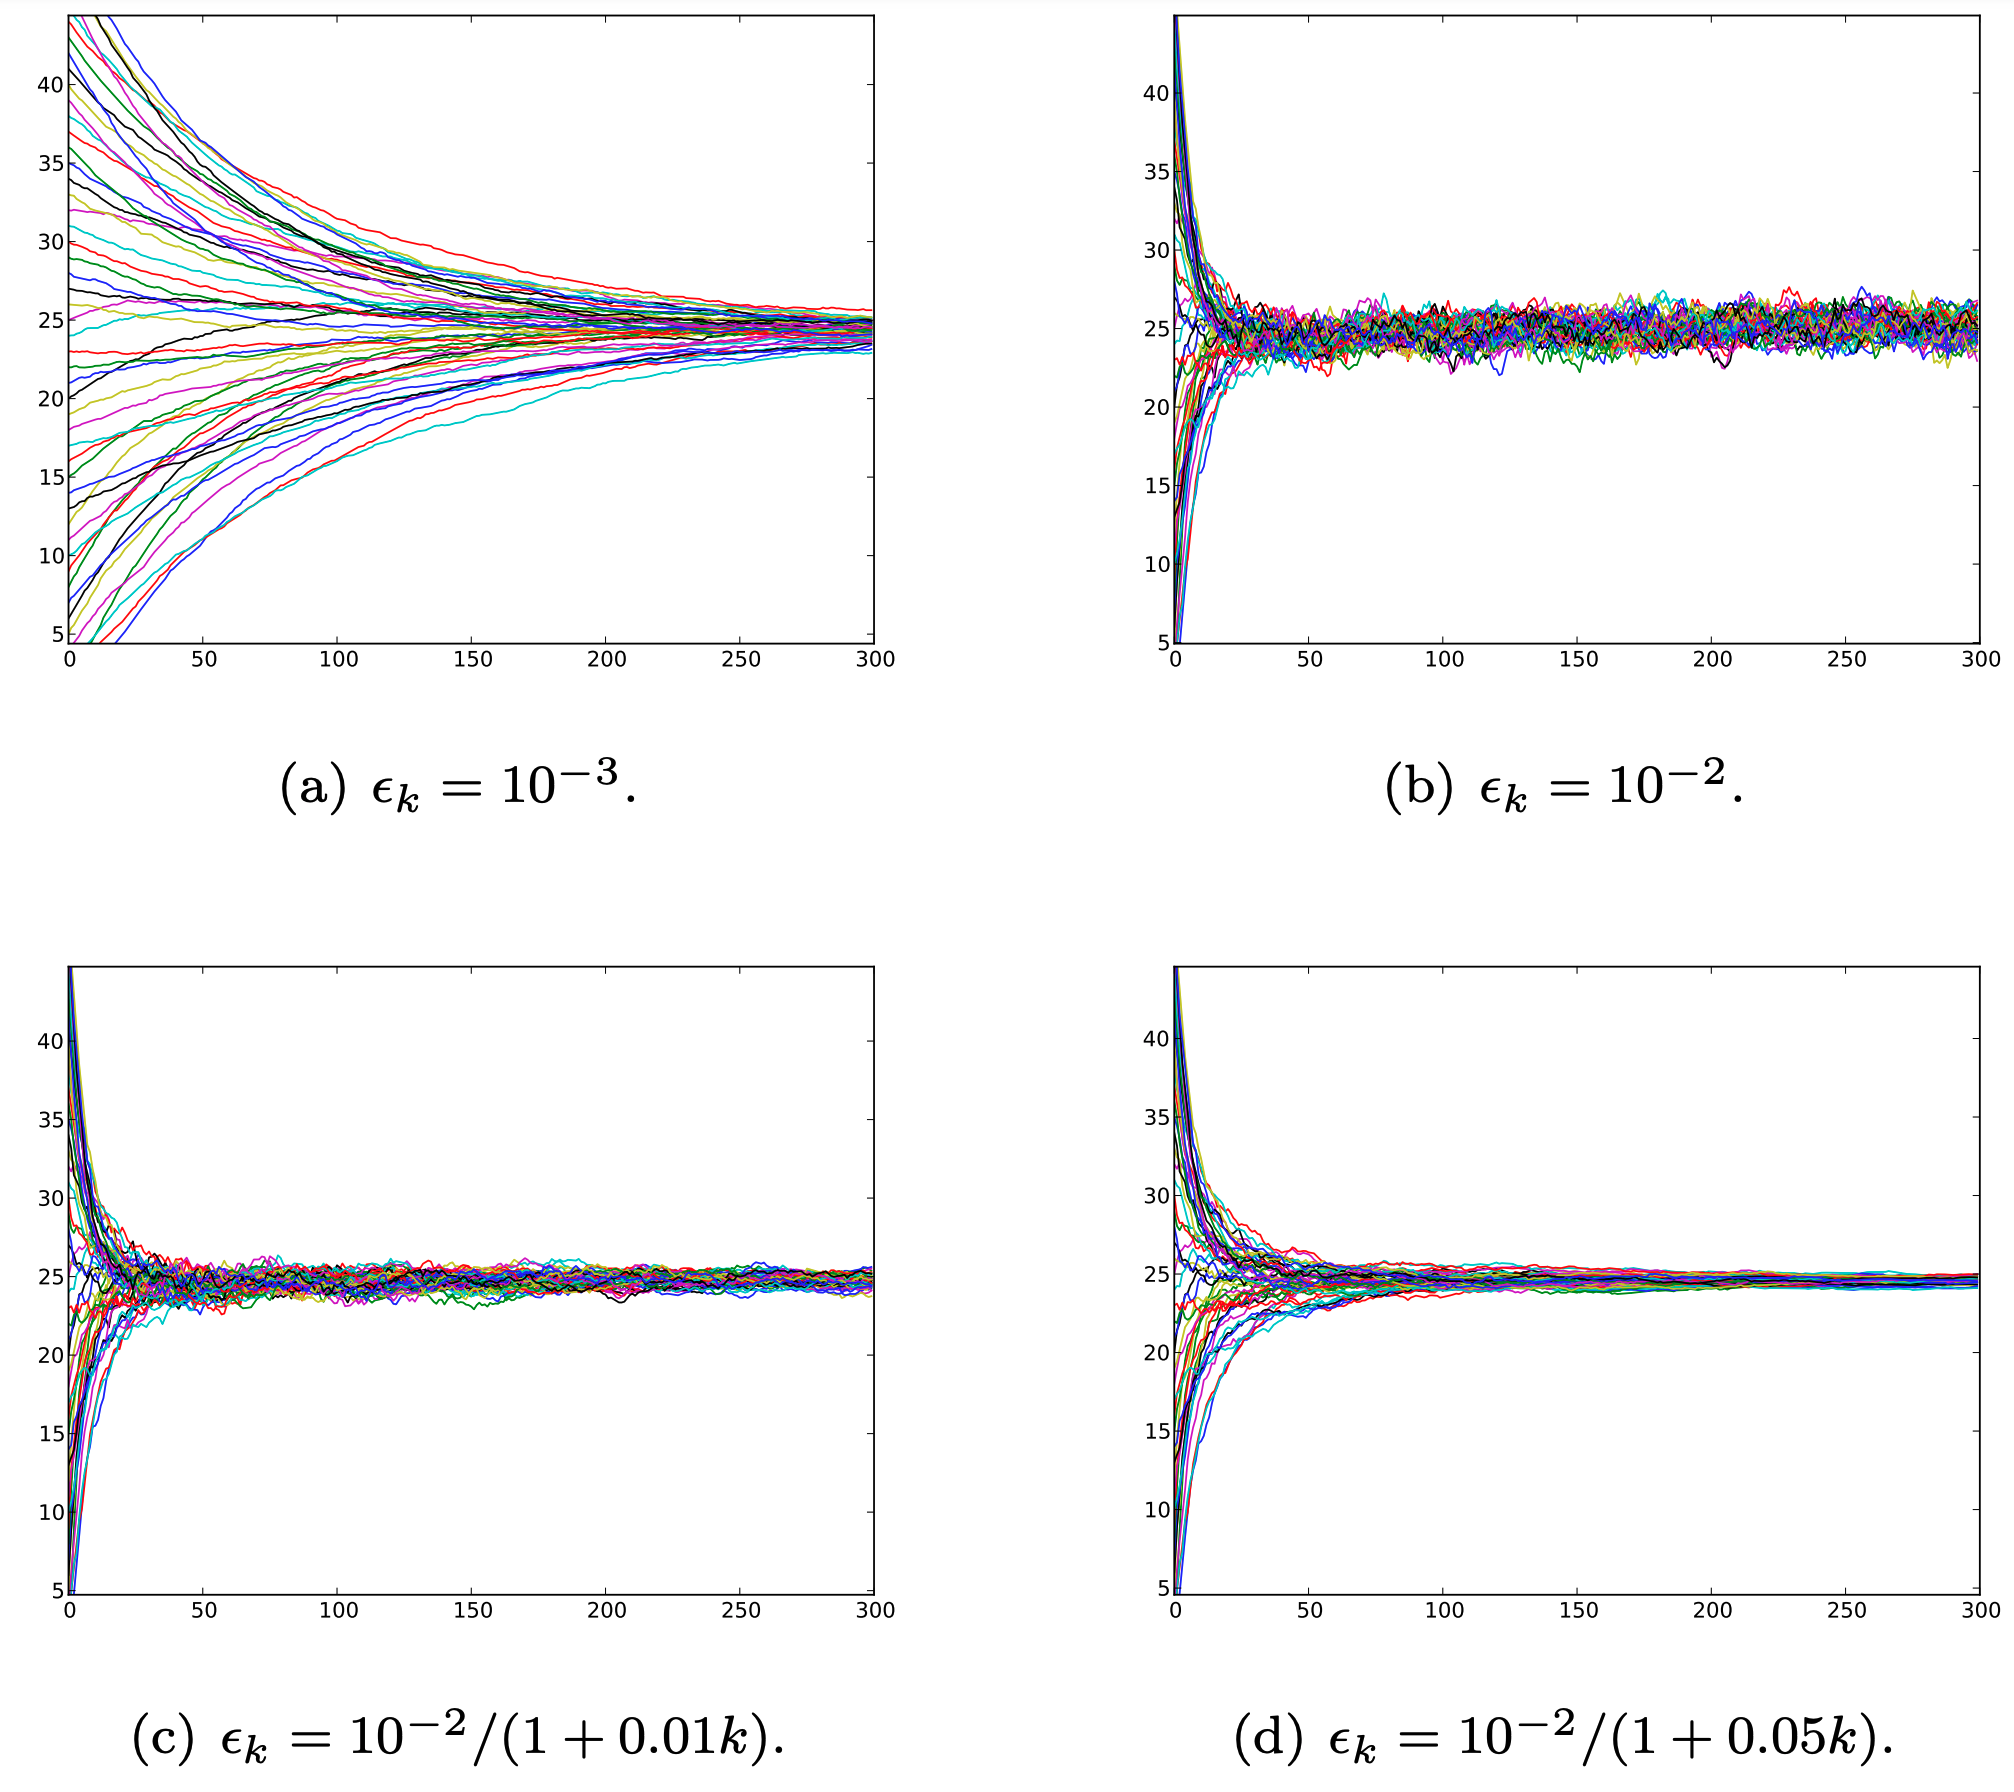
\includegraphics[scale=0.25]{conv.png}
%     \caption{\scriptsize Altering step-sizes to generate convergence trajectories.}
%     \label{fig:convergence-results}
% \end{figure}
    
\end{frame}
% % \section{Multi Time Scale approaches}
\section{Task 02: Content (Tweet) Generation}
\begin{frame}{Task 02: Content (Tweet) Generation}
    % To find the minima of a function we use Gradient Descent but scenarios where we do not have access to the gradient of the $f$ directly but only a noisy version of it, we can use SA as:
    % \begin{equation}
    %     \label{eq:sgd}
    %     x_{n+1}=x_n+\alpha_n\left[-\nabla f\left(x_n\right)+\mathbb{M}_{n+1}\right]
    % \end{equation}
    
    % which converges to the limiting ODE: $$\dot{x}(t)=-\nabla f(x(t))$$.
    % To account for a more generalized function which might not be smooth and noisy gradients must be replaced with noisy sub-gradients as given by the Kiefer-Wolfowitz procedure\cite{Bhatnagar2013} :
 
        
    %     $$x_{n+1}^i=x_n^i+\alpha_n\left[-\left(\frac{f\left(x_n+\delta e_i\right)-f\left(x_n-\delta e_i\right)}{2 \delta}\right)+\mathbb{M}_{n+1}^i\right]$$

    
\end{frame}

\section{Future Scope}
\begin{frame}{Future Scope: Psychographic Clustering}
    \begin{itemize}
        \item Psychographic clustering is the process of categorizing persons according to psychological and social criteria, such as their interests, values, lifestyles, and personalities.
        \item Segmentation goes beyond psychographic clustering by splitting the audience into discrete subgroups that have similar traits. Segmentation is a crucial component in constructing resilient prediction models. By comprehending the varied tastes among groups, we may customize our models to achieve more accuracy and personalization.
        \item Forecasting the number of likes by analyzing tweet metadata. Traditional models typically take into account variables such as posting time, frequency, and content kind. However, psychographic segmentation adds an additional level of complexity by integrating user preferences, emotions, and contextual comprehension.
    \end{itemize}
\end{frame}

% \begin{frame}{}
% \begin{figure}
%     \centering
%     \scriptsize
%     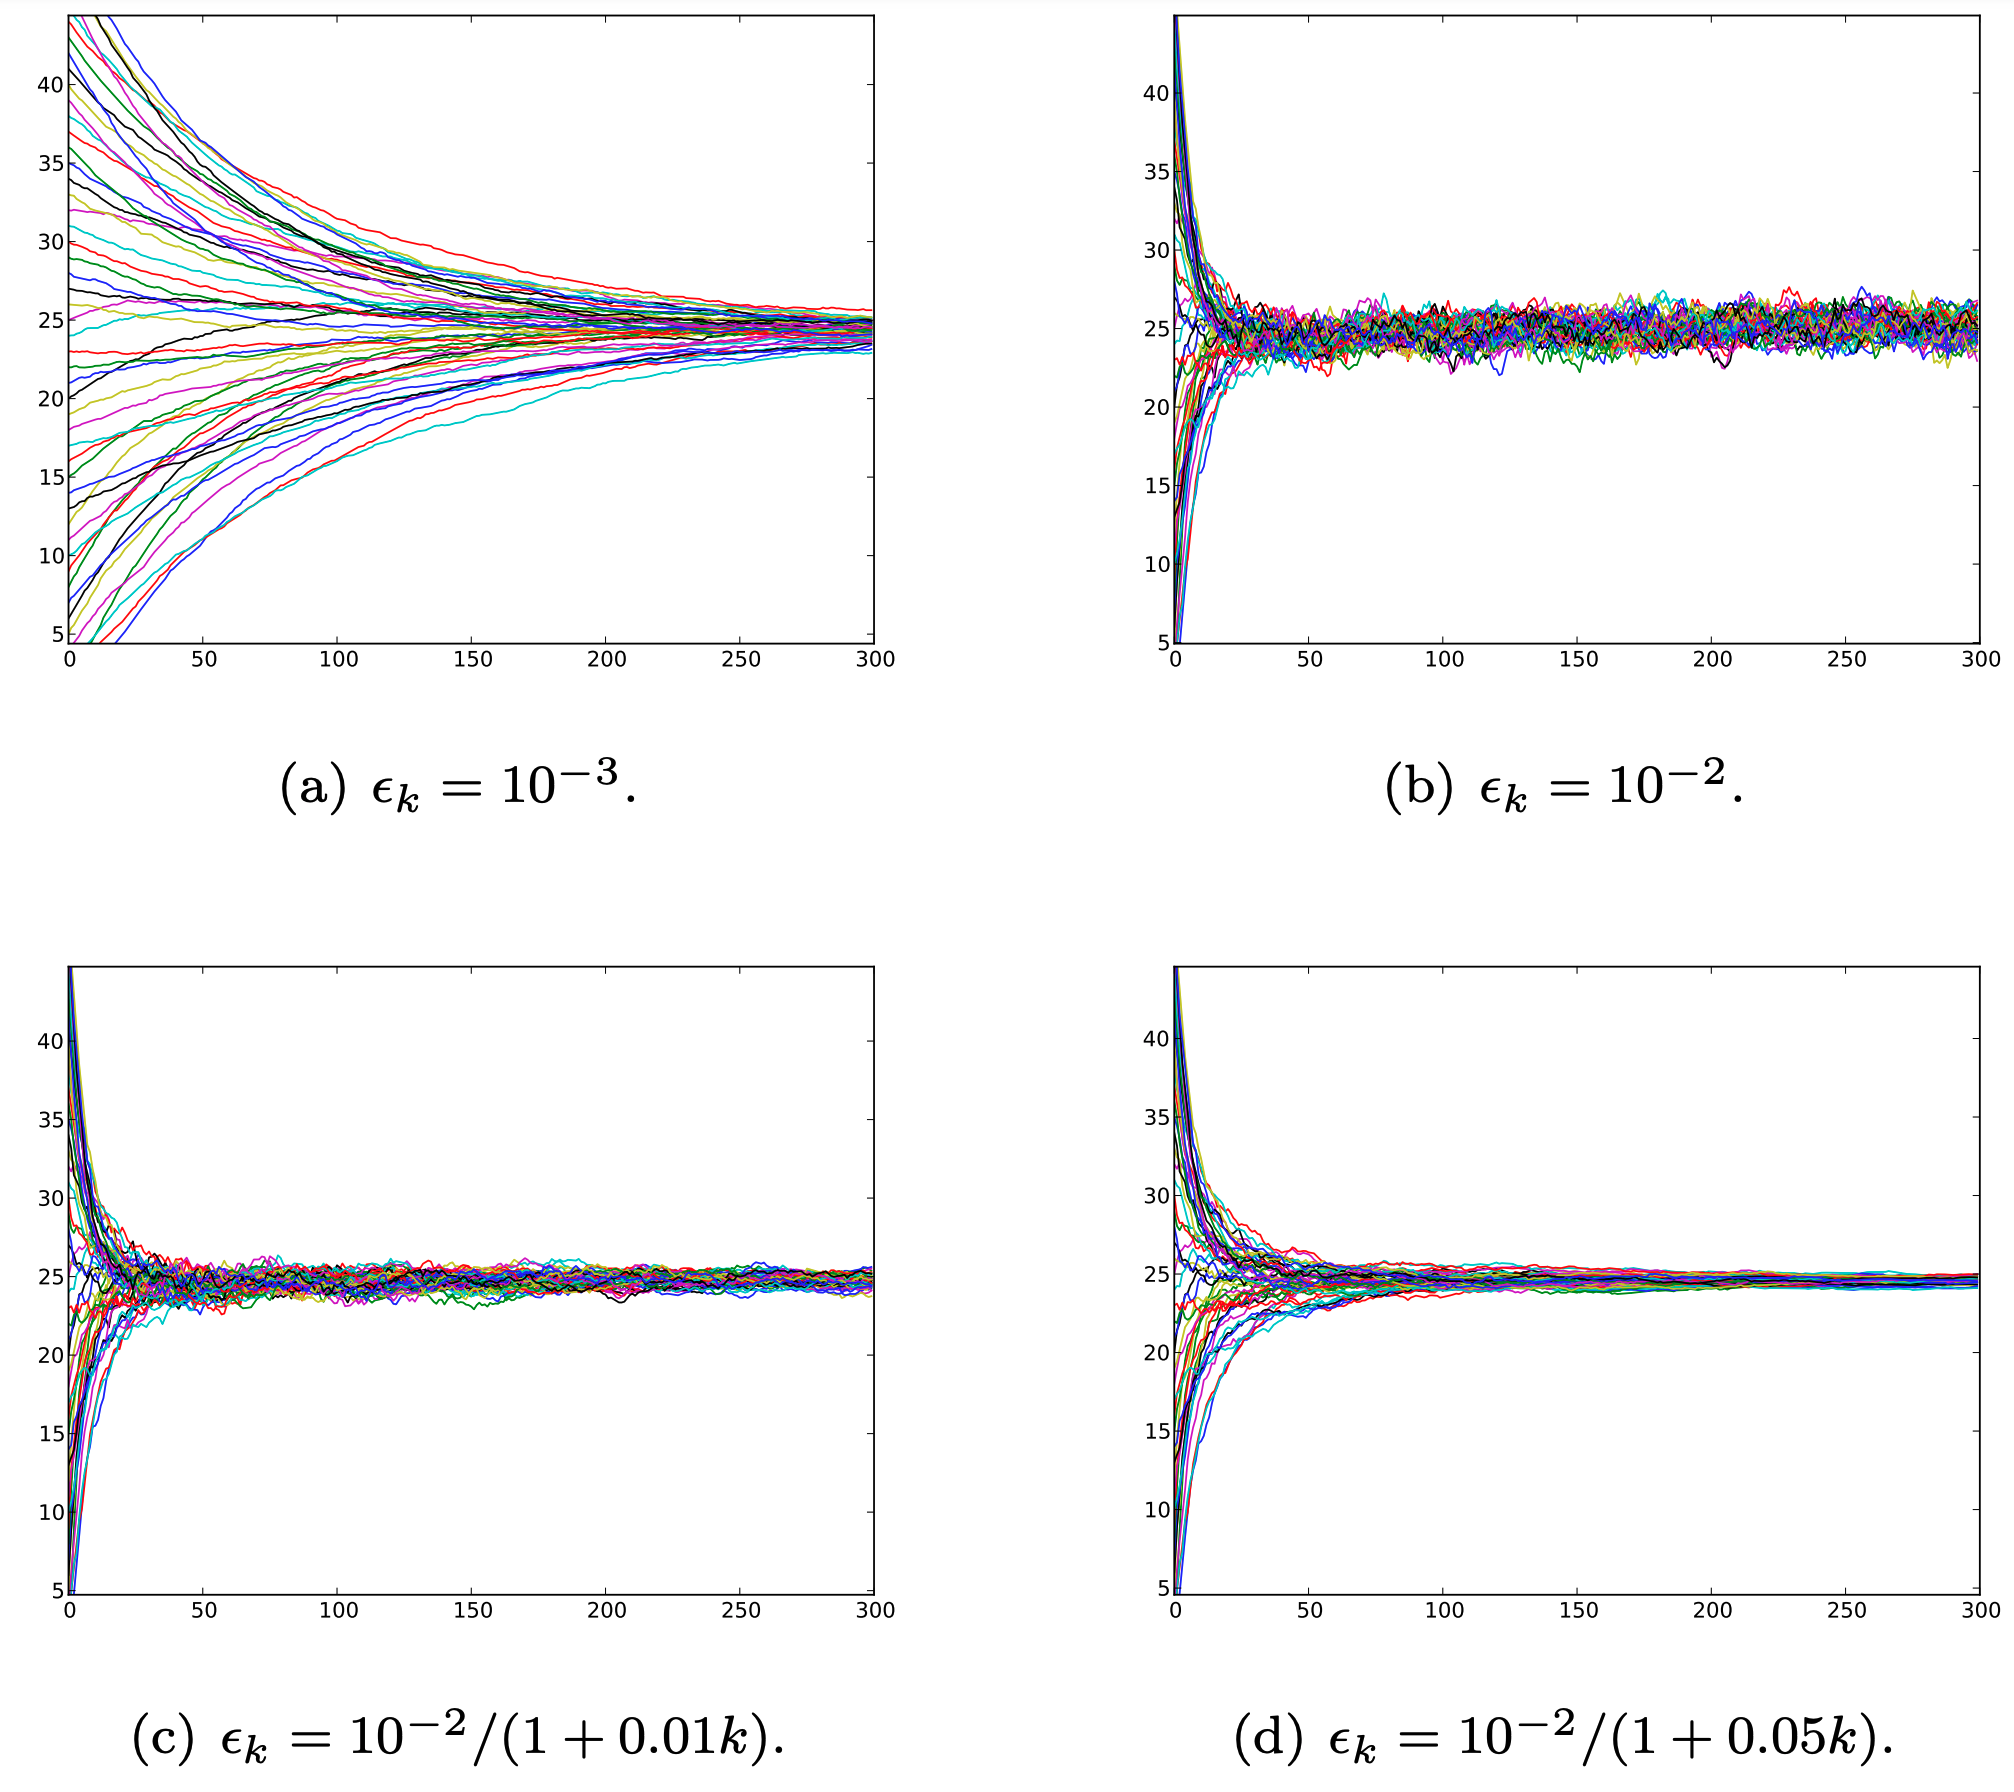
\includegraphics[scale=0.25]{conv.png}
%     \caption{\scriptsize Altering step-sizes to generate convergence trajectories.}
%     \label{fig:convergence-results}
% \end{figure}
    
% \end{frame}

\section{Conclusion}
\begin{frame}{Conclusion}
%     \begin{block}{Basic Convergence Analysis}
%         The stochastic recurrence given as $x_{n+1} = x_n + \epsilon_n (h(x_n) + \mathbb{M}_{n+1}); n\geq0 \,\, and \,\, x_0$ can be random and with above assumptions being true and $h(x)$ is Lipschitz continuous then the iterates ${x_n}$ track a.s. asymptotically the ODE \cite{borkar1998stability} $$\dot{x}(t)=h(x(t)), t \geq 0$$
%     \end{block}
% \end{frame}
% \begin{frame}{}
% \begin{figure}
%     \centering
%     \scriptsize
%     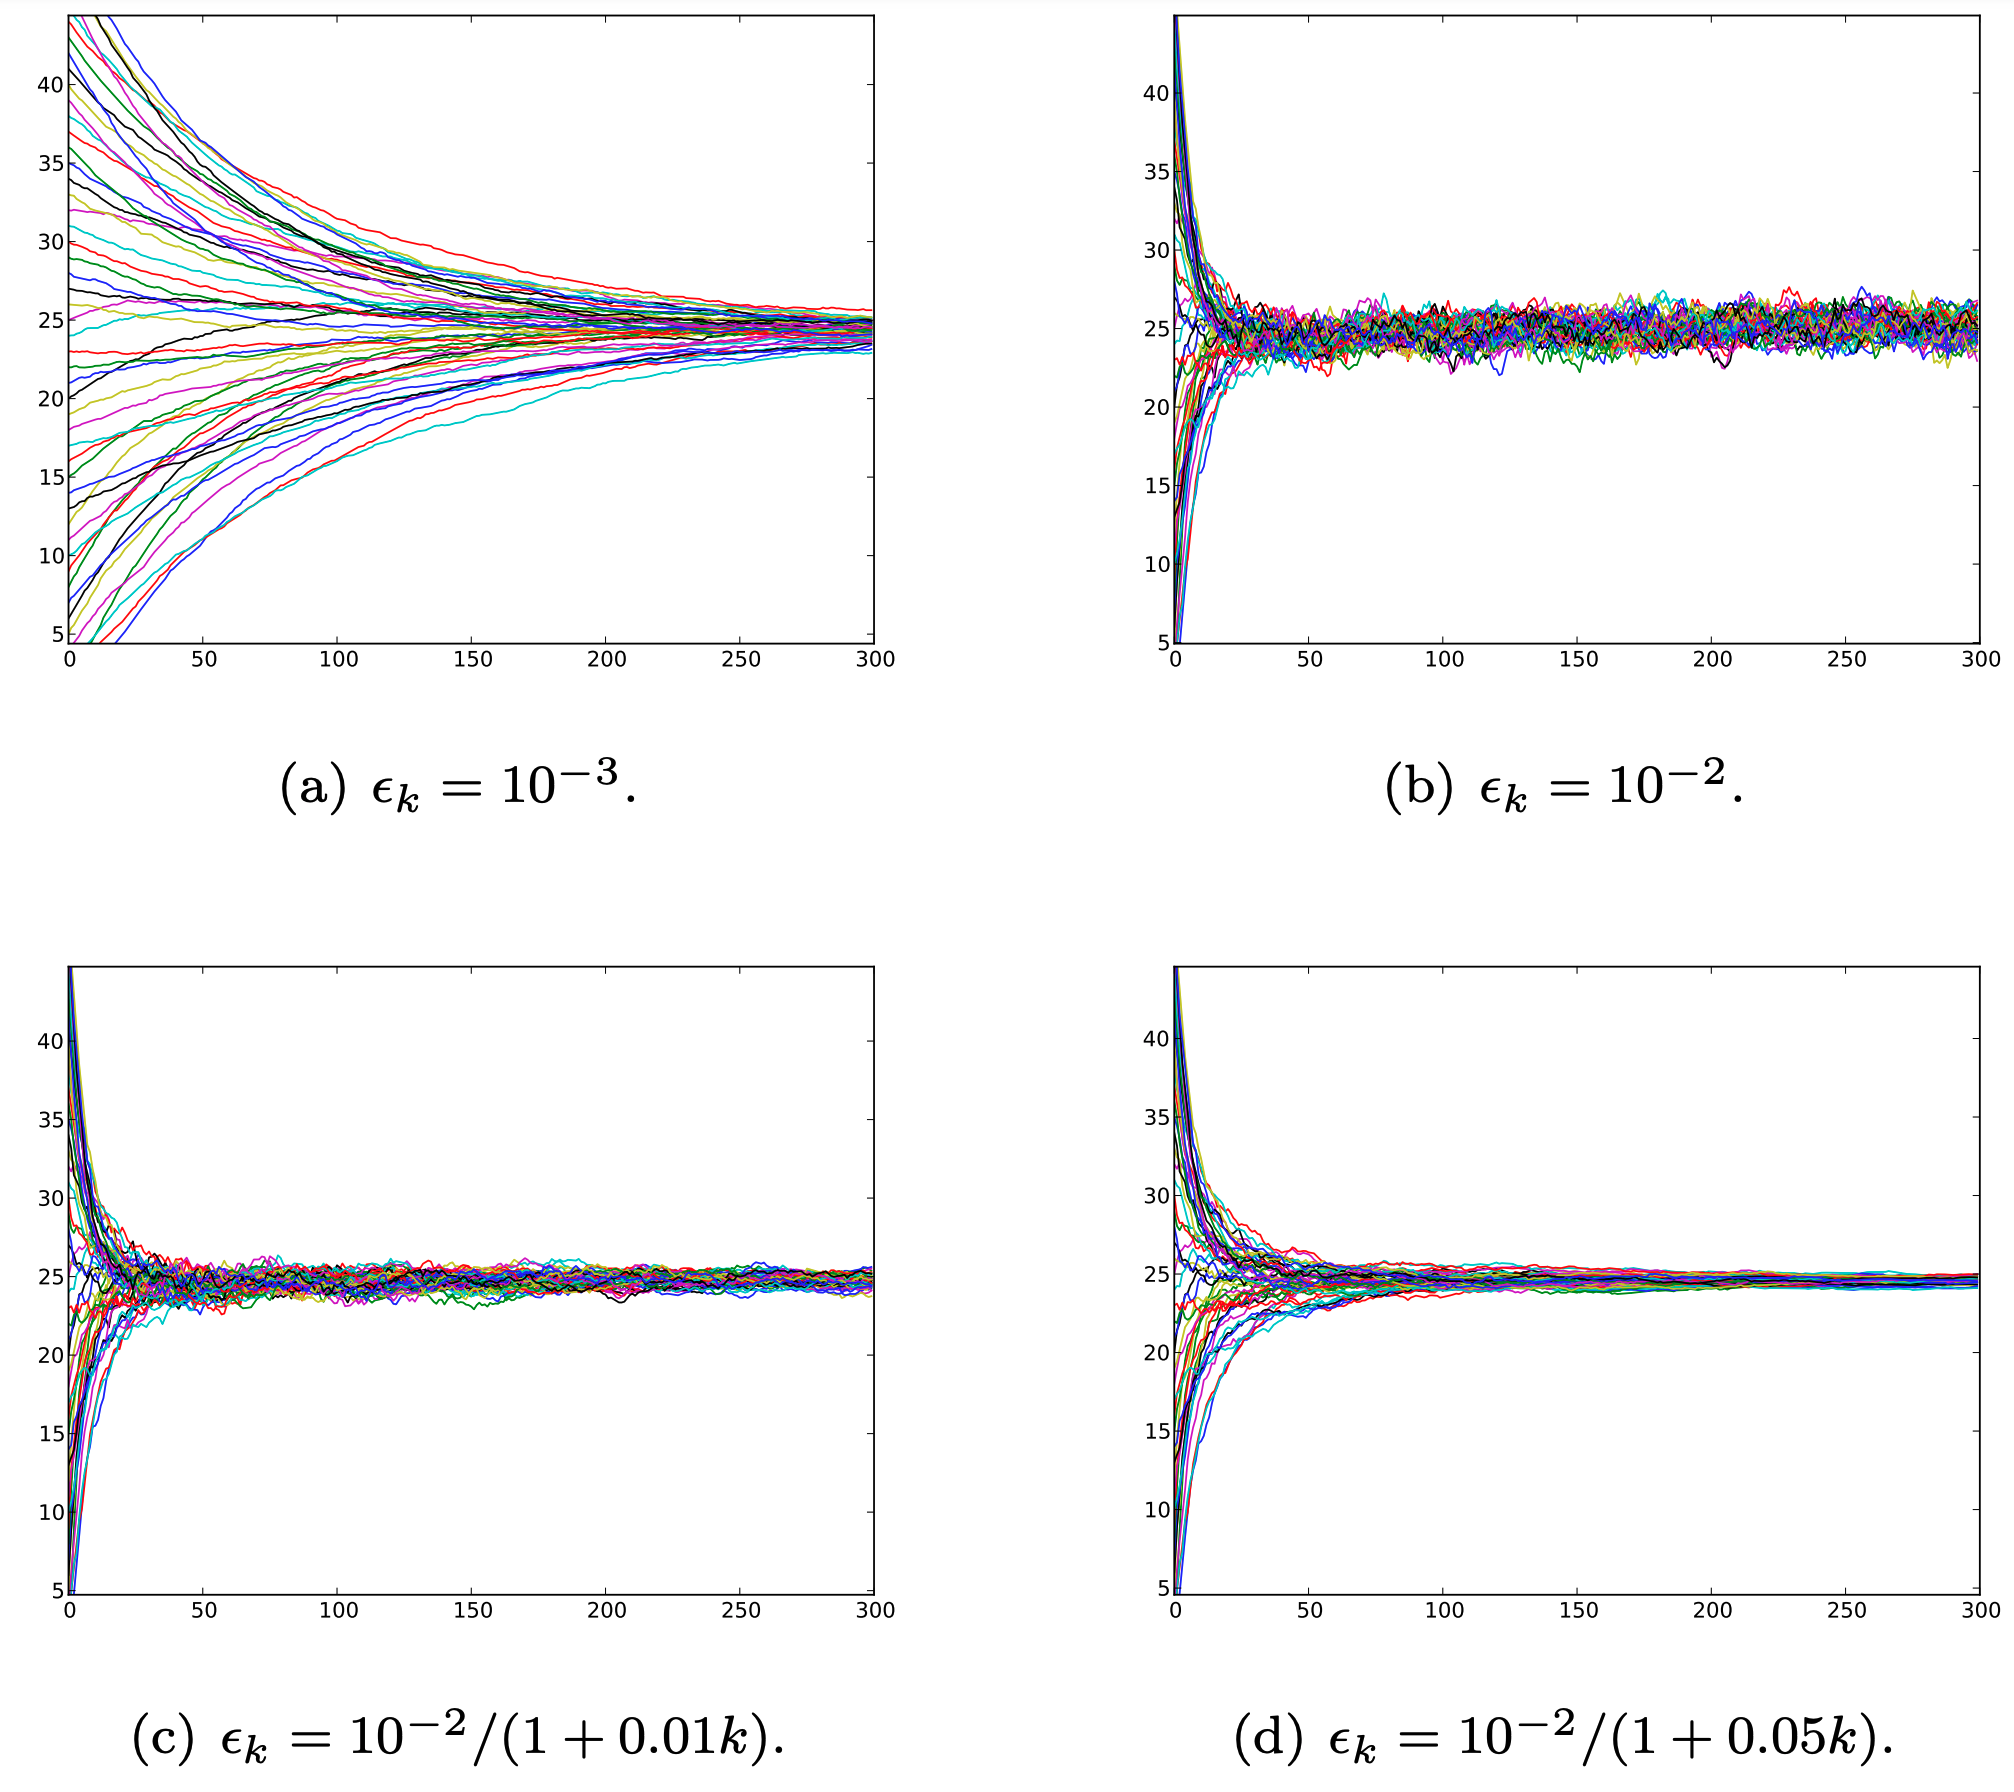
\includegraphics[scale=0.25]{conv.png}
%     \caption{\scriptsize Altering step-sizes to generate convergence trajectories.}
%     \label{fig:convergence-results}
% \end{figure}
    
\end{frame}

% \begin{frame}{Optimization of Expectation of Performance Measure}
% \scriptsize
%     For a given performance measure $J$ of some parameter $\theta$,  and X is r.v. with distribution $F_\theta$, then our problem:
%     $$ \min J(\theta) = \mathbb{E}_\theta[f(X)]
%     $$
%     Now it is typically difficult to compute $J(\theta)$, but if we fix $\theta=\theta_n$, we can generate samples $f(X)$ with $X$ distributed according to $F_{\theta_n}$. 
%     Now $\Lambda_\theta(x)$ being the likelihood-ratio which is continuously differentiable in $\theta$, 
% $$
% J(\theta)=\int f(x) d \mu_\theta(x)=\int f(x) \Lambda_\theta(x) d \mu(x) ; 
% $$
% If the interchange of expectation and differentiation can be justified, then
% $$
% \frac{d}{d \theta} J(\theta)=\int f \frac{d}{d \theta} \Lambda_\theta d \mu
% $$
% and the stochastic approximation
% \begin{equation}
%     \label{eq:expperf}
%     \theta_{n+1}=\theta_n+\gamma_n\left[\left.f\left(X_{n+1}\right) \frac{d}{d \theta} \Lambda_\theta\left(X_{n+1}\right)\right|_{\theta=\theta_n}\right]
% \end{equation}


% and \ref{eq:expperf} will track the ODE
% $$
% \dot{\theta}(t)=\frac{d}{d \theta} J(\theta)
% $$
% \end{frame}

% \begin{frame}{Stochastic Fixed Point Iterations}
%     A stochastic approximation of the form
% \begin{equation}
%     \label{eq:fixed}
%     x_{n+1}=x_n+\alpha_n\left[F\left(x_n\right)-x_n+\mathbb{M}_{n+1}\right]
% \end{equation}


% can be used to converge to a solution $x^*$ of the equation $F\left(x^*\right)=x^*$, i.e., to a fixed point of $F$. The limiting ODE of \ref{eq:fixed}  is
% $$
% \dot{x}(t)=F(x(t))-x(t)
% $$
% We consider the case where $F$ is an $\gamma$-contraction $(0 \leq \gamma<1)$ with respect to a weighted norm on $\mathbb{R}^d$
% $$
% \begin{aligned}
% \|x\|_{p, w} & :=\left(\sum_{i=1}^d w_i\left|x_i\right|\right)^{1 / p}, \\
% \text { or }\|x\|_{\infty, w} & :=\max w_i\left|x_i\right|
% \end{aligned}
% $$
% \end{frame}

% \begin{frame}{Q-Learning}
% \scriptsize
%     In a Reinforcement Learning setting we are often faced with the Q-Learning update as follows:
    
% \begin{equation}
%     \label{eq:qlearning}
%     Q_{k+1}\left(S_k, A_k\right)=Q_k\left(S_k, A_k\right)+\epsilon_k\left[\mathcal{R}\left(S_k, A_k\right)+\gamma \max _{a \in \mathcal{A}} Q_k\left(S_{k+1}, a\right)-Q_k\left(S_k, A_k\right)\right]
% \end{equation}
% \begin{itemize}
%     \item convergence is efficiently estimated using SA framework to find the optimal $Q^*$ such that $\argmax Q^* = \pi^*$.
%     \item The sequence $Q_k$ generated by $Q$-learning converges to $Q^*$ w.p. 1 as long as every state-action pair is visited infinitely often under the sampling policy $\pi$, and the step size diminishes to zero at a proper rate.
% \end{itemize}
% For settings where state-action pair space is huge we can project it to lower dimensional linear subspace and the SA algorithm is still valid which takes the form : 
%     \begin{equation}
%     \label{eq:linfuncapprox}
%         \theta_{k+1}=\theta_k+\epsilon \phi\left(S_k, A_k\right)\left[\mathcal{R}\left(S_k, A_k\right)+\gamma \max _{a \in \mathcal{A}} \phi\left(S_{k+1}, a\right)^{\top} \theta_k-\phi\left(S_k, A_k\right)^{\top} \theta_k\right]
%     \end{equation}


% \end{frame}

% \begin{frame}{Two time scale SA : Actor-Critic Algorithms}
% \begin{figure}
%     \centering
%     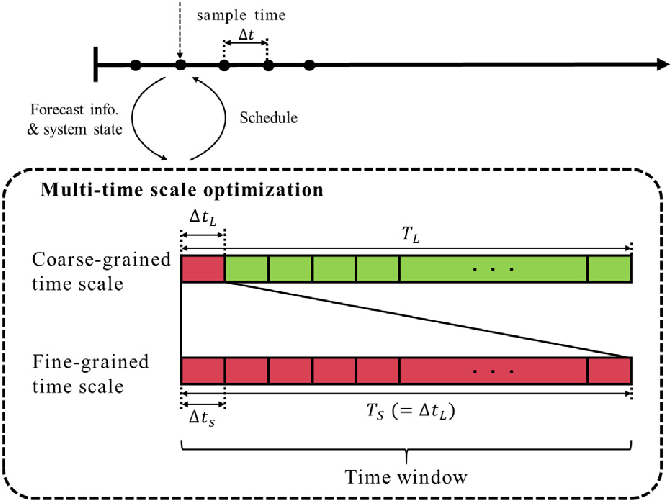
\includegraphics[scale=0.28]{mutlitime.png}
%     \caption{\scriptsize Illustration of multi time scale approach, where w.r.t the faster time scale the slower one is quasi-stationary.}
%     \label{fig:multitime}
% \end{figure}
    
% \end{frame}
% \begin{frame}{}
%     Now we consider a two-scale version of the same SA framework:
%     \begin{equation}
%         \begin{aligned}
% & X_{n+1}=X_n + \alpha_n(F(X_n, Y_n)+\mathbb{M}_{n+1}) \\ \\
% & Y_{n+1}=Y_n + \beta_n\left(G(X_n, Y_n)+\mathbb{M}^{\prime}_{n+1}\right)
% \end{aligned}
% \label{eq:multitime}
%     \end{equation}
%     Where all the above assumptions apply for the noise and the functions $F$ and $G$ also the step-sizes are decayed and staggered and the slower rate is quasi-static w.r.t faster rate.

% \end{frame}
% \begin{frame}{}
%     \begin{figure}
%         \centering
%         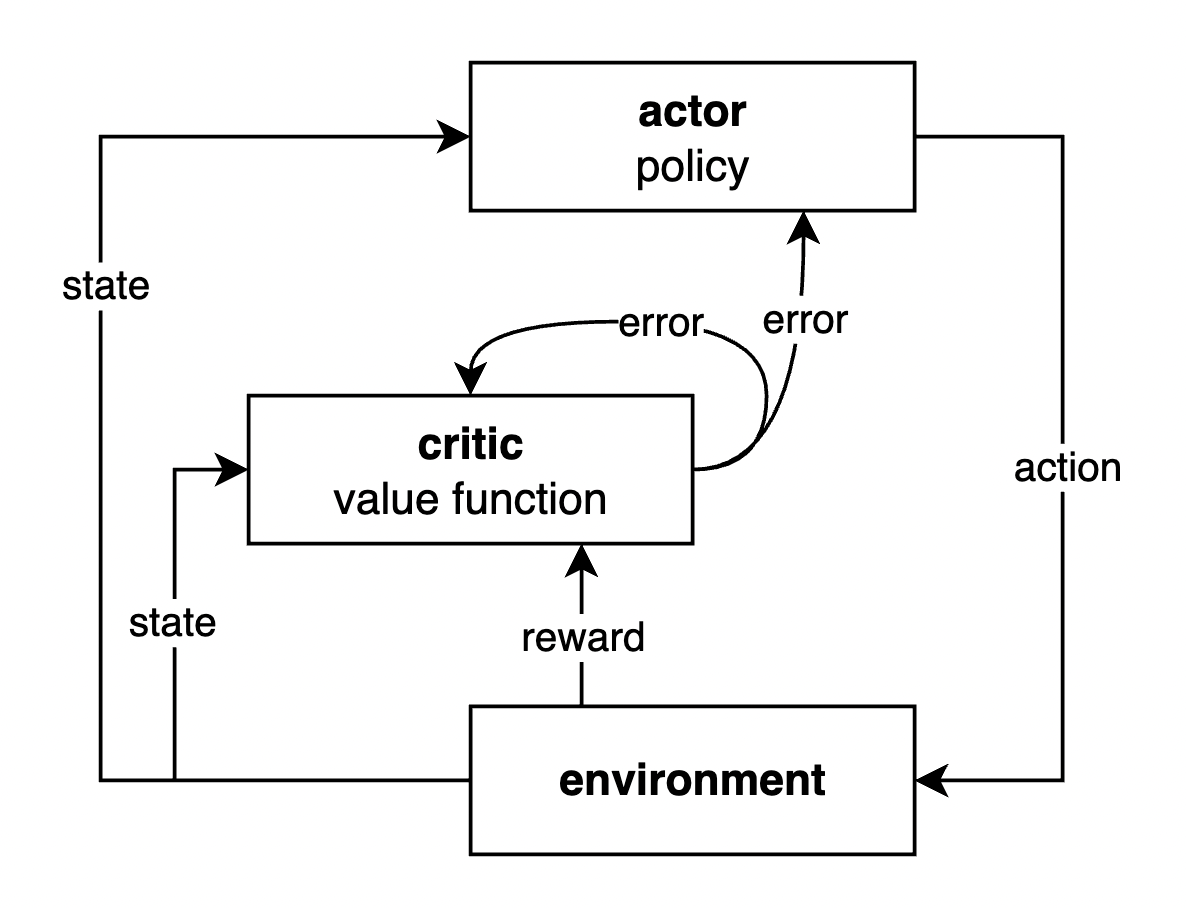
\includegraphics[scale = 0.2]{ac.png}
%         \caption{Actor-Critic Architecture - the actor and the critic are updated simultaneously at each iteration except that the actor changes more slowly (with a small step size) than the critic (with a large step size).}
%         \label{fig:enter-label}
%     \end{figure}
%     \scriptsize
    
% \end{frame}
% \section{Conclusion}
% \begin{frame}{Conclusion}
% \justifying
%     \begin{itemize}
    
%         \item Renewed interest has been ushered in the stochastic approximation as it fundamental for the convergence of many RL and other adaptive learning algorithms.
%         \item The fundamental form being a recursive stochastic difference equation can be easily modelled and simulated.
%         \item Convergence of algorithms can be controlled using appropriate step size updates.
%     \end{itemize}
    
% \end{frame}

% \begin{frame}[allowframebreaks]
%         \scriptsize
      
%         \frametitle{References}
%         \bibliographystyle{IEEEtranN}
%         \bibliography{ref.bib}
% \end{frame}

% \begin{frame}{}
%     \centering \Large
%     \emph{Thank You}
% \end{frame}
\end{document}